% % % % % % % % % % % % % % % % % Preamble for notes % % % % % % % % % % % % % % % % % % % % % % % %
\documentclass[12pt,oneside,a4paper]{article}


% % % % % Sprogpakker og Layout % % % % % % % % %
\usepackage[left=2.5cm,top=2.0cm,bottom=1.5cm, right=3.0cm]{geometry}
\usepackage{ulem}
\usepackage[danish,english]{babel}
\usepackage[utf8]{inputenc}
\linespread{1.3}       % simulerer Word 1.5 line spacing

% % % % % % % % % % Øvrige vigtige pakker % % % % %
\usepackage{graphics}
\usepackage{amsmath}
\usepackage{amssymb}
\usepackage{url}
\usepackage{cancel}
\usepackage{booktabs}
\usepackage{pdfpages}
\usepackage{mathpazo}
\usepackage[section]{placeins}
\usepackage{caption}
\usepackage{wrapfig}
\usepackage{tocloft}
\usepackage{subfig}
\usepackage{fancyhdr}
%Muliggør 'flere figurer i én' Eksempel på anvendelse (indenfor figure-environment):
% \subfloat[undercaption 1]{\label{label 1}\includegraphics[bredde 1]{billede 1}}
% \subfloat[undercaption 2]{\label{label 2}\includegraphics[bredde 2]{billede 2}}
% \caption{overordnetcaption}
% \label{overordnet label}
\usepackage{lscape}
%Omdanner en del af dokumentet til landscape. Angives med \begin{landscape}
\usepackage{framed}
%Sætter en ramme om et område begrænset af \begin{framed} og \end{framed}.
%Allows footnotes
\usepackage{footnote}
\setlength{\parindent}{0cm}
\setlength{\parskip}{0.3cm}
% % % % % % COMMANDS % % % % % % % %

\numberwithin{equation}{section}
\begin{document}

\selectlanguage{english}
% % % % % % % % % % % % % % % % % % % % % % Forside % % % % % % % % % % % % % % % % % % % % % % % % %
\pagenumbering{roman}

\begin{center}
{\textsc {\LARGE \bf{Københavns Universitet \\[0.3cm]  Bachelorstudiet i fysik}}}\\[1.5cm]
{\textsc {\Large \bf Førsteårsprojekt 2017}}\\[0.8cm]
{\Large Projekt nummer: 2017-06}\\[1cm]

\rule{15cm}{0.01cm}\\[1cm]
{\LARGE\bf  Bouncing ball}\\ [0.5cm]
\rule{15cm}{0.01cm}\\[1cm]
\end{center}

\vfill
{\large Forfattere:}\\
{\large \hspace*{1cm} \makebox[6cm][l]{Andreas M. Faber}  \hspace{1cm} KU- ID: \makebox[2cm][l]{QZJ517} \\
{\large \hspace*{1cm} \makebox[6cm][l]{Benjamin T. Søgaard}   \hspace{1cm} KU- ID: \makebox[2cm][l]{MGX877} \\
{\large \hspace*{1cm} \makebox[6cm][l]{Joachim J. Kønigslieb}   \hspace{1cm} KU- ID: \makebox[2cm][l]{GWC666} \\

{\large Vejledere:}\\
{\large \hspace*{1cm} \makebox[6cm][l]{Jörg Helge Müller}  \hspace{1cm} Email: \makebox[2cm][l]{muller@nbi.ku.dk} \\

\vfill

{\large Rapporten omfatter {\bf 1} siders hovedtekst og {\bf 1} siders appendix.}

{\large Rapporten er indsendt som en pdf-fil den 17 marts 2017. }

\normalsize


% % % % % % % % % % % % % % % % % % % % % % Abstract  og Indholdsfortegnelse % % % % % % % % % % % % % % % % 
\newpage
\begin{abstract}
Kort resumé, gerne på både dansk og engelsk.
\end{abstract}

\newpage

\tableofcontents


% % % % % % % % % % % % % % % % % % % % % % Indhold % % % % % % % % % % % % % % % % % % % % % % % % %
\newpage
\pagenumbering{arabic}
\section{Introduction to chaos}

asdfagaffhåijpsfgh

\section{The experiment}

\section{Model of the system}
\subsection{General model}
We will model our experiment as a 1-dimensional system that is we will not account for sideways motion. On figure \ref{bounces} two consecutive bounces can be seen where the later is bigger due to the plate  moving upwards at the time of impact.
\begin{figure}[h]
	\centering
	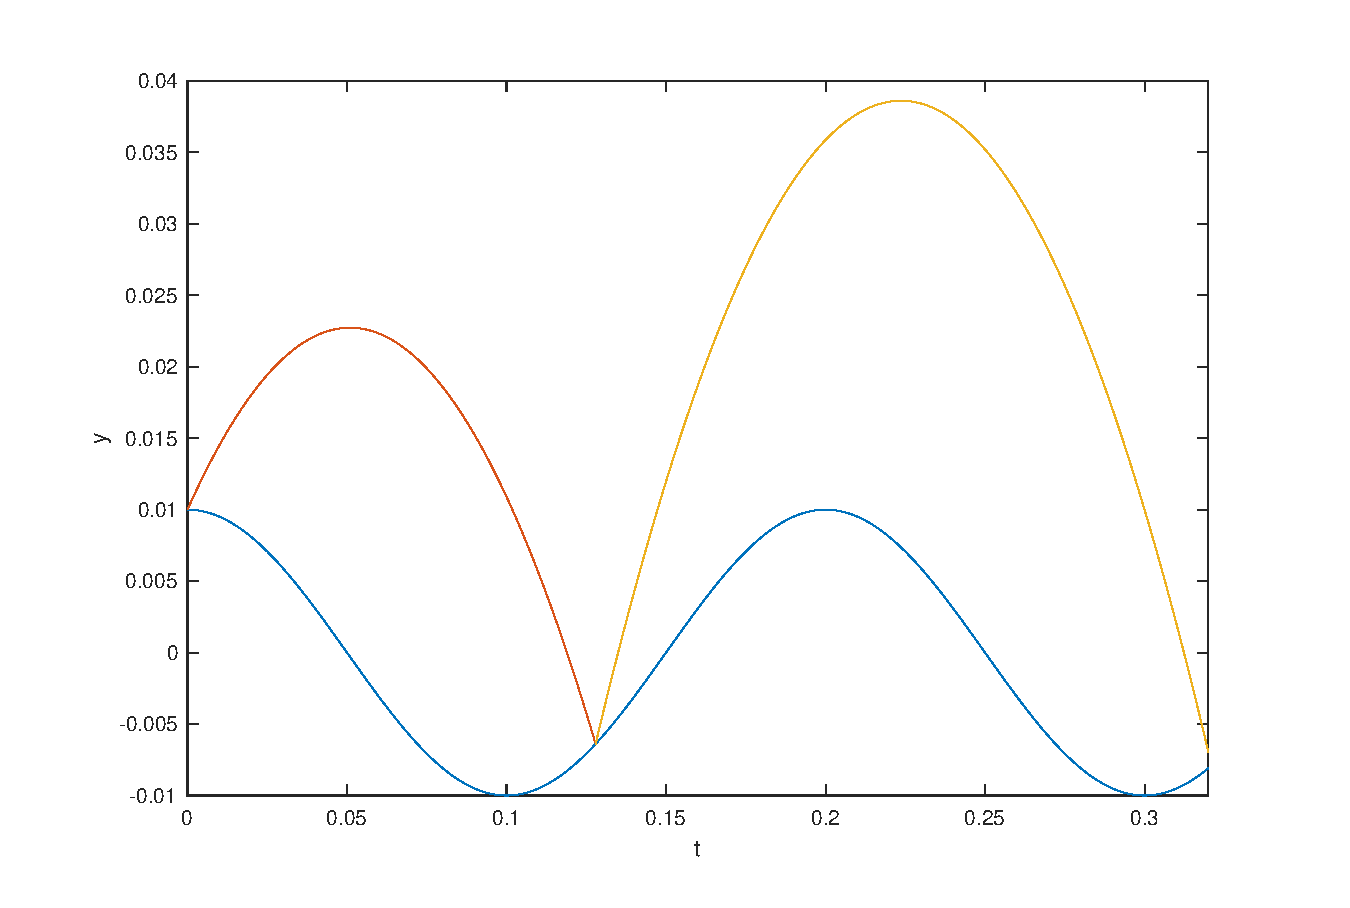
\includegraphics[width=0.6\textwidth]{Figures/bounceplot.eps}
	\caption{Plot of two bounces on the vibrating plate}
	\label{bounces}
\end{figure}
The $k^{\text{th}}$ bounce can be completely described by the time $t_k$ it left the plate and the velocity $v_k$ at that instance. Time and phases $\phi_k$ can be used interchangeably through the relationship $\phi=2\pi f t$.

To describe the system during a specific bounce we denote the distance of the ball above the plates rest position $y_b(t)$. Similarly we define $y_p(t)$ as the displacement of the vibrating  plate from it equilibrium. For a given frequency $f$, phase shift $\phi$ and amplitude $A$ the equation of motion for the plate is
\begin{equation}
	y_p(t)= A \sin(2\pi f t+ \phi)
	\label{platey}
\end{equation}
In air the ball is essentially a body in free fall, and since it is quite small and dense, the air resistance can be ignored. Thus the equation of motion for the ball $y_b(t)$ for the $k^\text{th}$ jump has the initial conditions $v_k$, $y_p(t_k)$ at time $t_k$, simply is
\begin{equation}
	y_{b,k}(t) = -\frac{g}{2}(t-t_k)^2+v_k(t-t_k)+y_p(t_k)
	\label{ybeq}
\end{equation}
For each jump we will denote the change of in initial $y$-coordinate\footnote{In general it is not possible to find $\Delta y_k$ analytically as it would require one to find the intersection between the graph of a parabola and a sine wave.} as $\Delta y_{k}=y_p(t_{k+1})-y_p(t_{k})$. Plugging that into (\ref{ybeq}) and solving for $t$ determines the fly time of each jump.
\begin{equation}
	\Delta t_{k} = t_{k+1}-t_{k} = \frac{v_{k}+\sqrt{v_k^2-2g\Delta y_k}}{g}
\end{equation}
Futher we can derive equation (\ref{ybeq}) finding the velocity of the ball thereby finding the final velocity for each jump $v_{k,f}$.
\begin{equation}
	v_{b,k}(t) = -g(t-t_k)+v_k \Rightarrow v_{k,f} = v_{b,k}(t_k+\Delta t_K) = -\sqrt{v_k^2-2g\Delta y_k}
\end{equation}
To model the impact between the ball and the plate we use a constant coefficient of restitution $C_r$ although more complex models have been suggested. For a plate at rest the velocity after the impact is proportional to the velocity before by $C_r$ such that $v_{up}=-C_r v_{down}$. For a moving plate we simplify transform into the coordinate system where the plate is at rest and then transform back. The veolicty of the plate is easily obtain by deriving (\ref{platey}).
\begin{equation}
	v_p(t) = -2\pi f A \cos(2\pi f t+ \phi)
\end{equation}
Putting the two together yields the following relationship between the final velocity of the $k^{th}$ jump $v_{k,f}$ and the initial velocity of the next $v_{k+1}$.
\begin{align}
	v_{k+1} &= -C_r(v_{k,f}-v_p(t_k+\Delta t_k))+v_p(t_k+\Delta t_k) \nonumber \\
	&= C_r \sqrt{v_k^2-2g\Delta y_k}-2(C_r+1)\pi f A \cos(2\pi f (t_k+\Delta t_k)+ \phi) \label{impactv}
\end{align}
Equation (\ref{impactv}) looks quite complicated as it is for the most general case, but as we shall see in the next section it can be used together with a number of assumptions.

\subsection{1-Period stable}
If we consider the most simple stable state of our system, it is when the ball is bouncing with identical trajectories. A more formal way of stating it is that $\Delta t_k$ should be constant. This  

% % % % % % % % % % % % % % % % % % % % % % Appendix % % % % % % % % % % % % % % % % % % % % % % % % %
\newpage
\appendix
\section{Derivation of the equations of motion for a driven harmonic oscillator}
The equation of motion for a driven simple harmonic oscilator will be of the form:
\begin{align*}
my'' + by' + ky = F\sin(\omega t)\\
y'' + \frac{b}{m}y' + \frac{k}{m} y = F \sin(\omega t)
\end{align*}
We will then write the general solution as a sum of the particular and the homogenues solutions:
\begin{align*}
y_g = y_{h} + y_p
\end{align*}
The homogeneous solution for the damped harmonic oscillator will go to zero with time. We claim it is only the particular solution that matters. To solve this, we will guess the solution to be of the form:
\begin{align*}
y_p = A \sin (\omega t) + B \cos(\omega t)
\end{align*}
We will perform the differentiation and plug into the equation to get:
\begin{align*}
&m\left(-A\omega^2\sin(\omega t) - B\omega^2\cos(\omega t)\right) + b\left(A\omega\cos(\omega t) - B\omega\sin(\omega t)\right) + k\left( A\sin(\omega t) + B\cos(\omega t) \right)\\
&=\sin(\omega t) \left( -mA\omega^2 -bB\omega + kA \right) + \cos(\omega t)\left(-mB\omega^2 + bA\omega + Bk\right)
\end{align*}
After collecting the coefficients, we can match the left side, with the right side:
\begin{align}
F &= -mA\omega^2 -bB\omega + Ak \label{lignA} \\ 
0 &= -mB\omega^2 + bA\omega + Bk \label{lignB}
\end{align}
We isolate an expression for $B$ in (\ref{lignB})
\begin{align*}
B &= \frac{-bA\omega}{-m\omega^2+k}
\end{align*}
Which we will proceed to plug into (\ref{lignA}), to obtain an expression for $A$:
\begin{align*}
A = \frac{F}{-m\omega^2+k+\frac{b^2\omega^2}{-m\omega^2+k}} = \frac{F\left(k-m\omega^2\right)}{\left(k-m\omega^2\right)^2+b^2\omega^2}
\end{align*} 
We can write $A$ and $B$ independetly of eachother:
\begin{align*}
B &= \frac{-bF\omega}{\left(k-m\omega^2\right)^2+b^2\omega^2}\\
A &=  \frac{F\left(k-m\omega^2\right)}{\left(k-m\omega^2\right)^2+b^2\omega^2}
\end{align*}
We would now like to express $y_p$ in the shape:
\begin{align*}
y_p = L \sin(\omega t + \phi)
\end{align*}
If we write the sine addition identity,
\begin{align*}
L sin(\omega t + \phi) = L\cos(\phi)\sin(\omega t) + L\sin(\phi)\cos(\omega t)
\end{align*}
We see, that our amplitude must obey,
\begin{align*}
A = L\cos(\phi)\\
B = L\sin(\phi)
\end{align*}
if we are to get our initial guess of
\begin{align*}
y_p = A \sin (\omega t) + B \cos(\omega t)
\end{align*}
The phaseshift will then be:
\begin{align*}
\frac{B}{A} &= \frac{L\sin(\phi)}{L\cos(\phi)} = \tan(\phi)\\
\phi &= \arctan\left(\frac{B}{A}\right)\\
\phi &= \arctan\left( \frac{-bF\omega}{\left(k-m\omega^2\right)^2+b^2\omega^2} \cdot \frac{\left(k-m\omega^2\right)^2+b^2\omega^2}{F\left(k-m\omega^2\right)} \right)\\
\phi &= \arctan\left( \frac{b\omega}{m\omega^2-k} \right)
\end{align*}
\end{document}
